\chapter{Data Transmitting and Platforms} \label{ch:platform}
The statistic data collected by a doorway counter is not of much use until it is analyzed. For a quick acquisition of data and a frequently updated overview of room occupancy, the count value should be sent to a remote platform at every time for further visualization and analyse.
\section{MQTT protocol}
We use MQTT (message queuing telemetry transport) to transfer data because it is supported by the ESP-IDF and widely accepted in IoT use cases. MQTT is an application layer protocol built on top of Wifi and TCP/IP. It is a light-weight, publish-subscribe network protocol, its structure is shown in \autoref{fig:mqtt}. When a publisher publishes, instead of sending to the receiver directly, the message is sent to a intermediate server called broker. Each message is published to a specific topic, a client would filter the messages by the subscribed topic and could only receive the message if it is listening to the same topic.

The light-weight usage of MQTT is mainly reflected by its transparent topic mechanism. A client does not need to create a topic before it publish or subscribe to it. A topic keeps alive when there is at least one publisher or subscriber. When a topic has at least one client on both pub/sub side, the data transmission becomes valid almost immediately. The topics in MQTT decouple the rigid connection between clients, reducing the complexity of connection drastically regardless of the scale (up to tens of thousands per MQTT server).

The main drawback of MQTT is no message buffering. A QoS (Quality of Service) setting higher than 0 on the client side only confirms that the message is received by the broker. If a message is published to a topic without listeners, that message is lost forever. Latest versions of MQTT supports retained messages, which stores one \emph{last known good value} in the broker. However, the retained messages aim to serve as a \emph{initialization default value} for those subscriber that join the topic between two publish intervals, storing more than one message is impossible. Secondly, MQTT is a queuing system instead of streaming, it delivers messages to a single consumer. When there are multiple consumers subscribing to a topic, they will consume the messages in a round-robin manner.
\begin{figure}
  \centering
  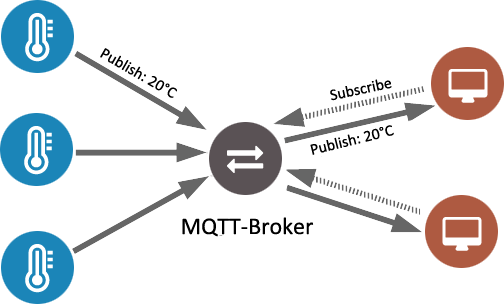
\includegraphics[width=0.6\textwidth]{figures/mqtt.png}
  \caption{MQTT network structure}\label{fig:mqtt}
\end{figure}
\section{Node-Red}
Visualization of an image frame sequence on websites often requires extensive programming. Fortunately, Node-Red \cite{nodered} relieves us from irrelevant affairs so that we can concentrate on the doorway counter development. Node-Red is a web-based visual programming editor that connects IoT devices or acts as an end-consumer. It supports message input from a MQTT broker, as well as http, websocket and serial. The smallest execution unit is called a node. A complete data process procedure consists of multiple nodes and is called a ``flow'', an example is shown in \autoref{fig:noderedflow}. Messages are propagated from flow start to flow end, and could be modified, truncated, merged with other flows, or splitted.
\begin{figure}
  \centering
  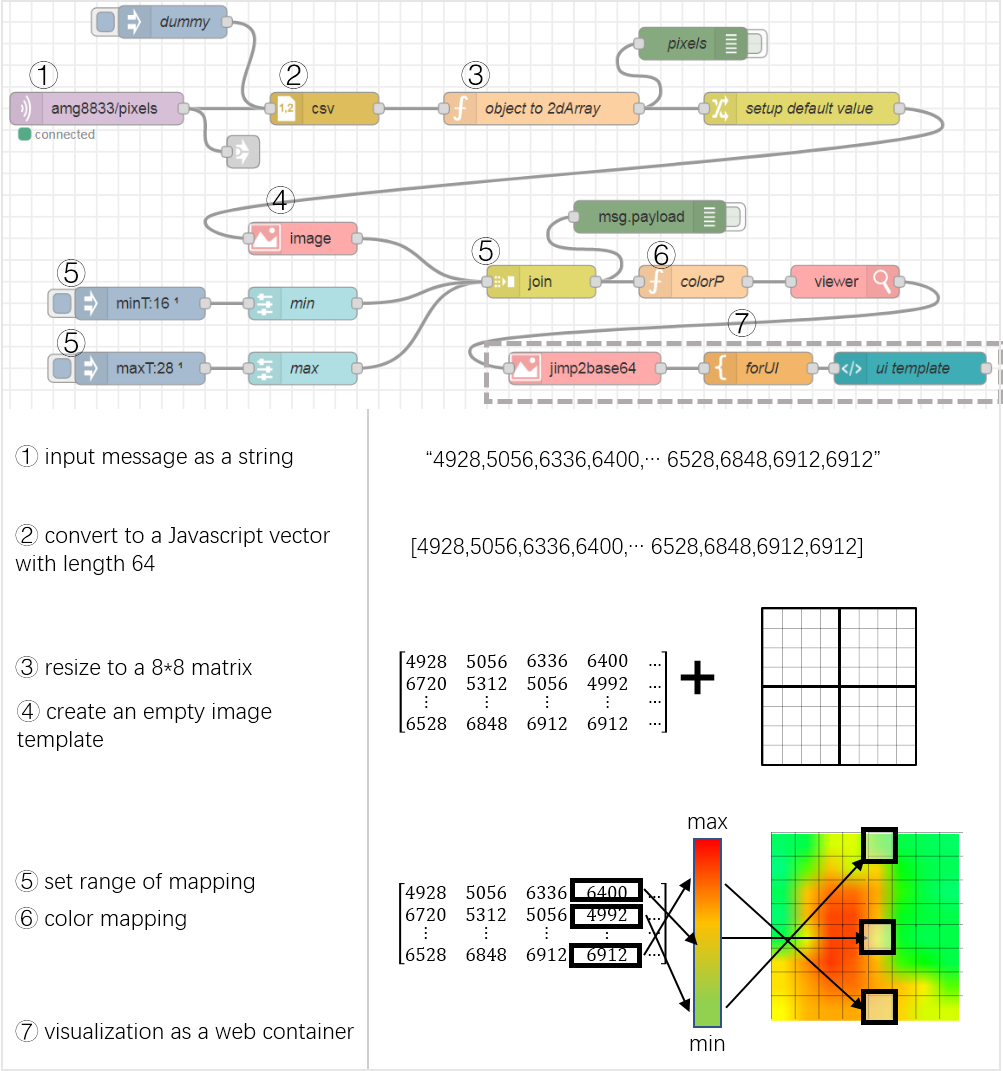
\includegraphics[width=0.8\textwidth]{figures/noderedflow.PNG}
  \caption{Our Node-Red flow used for $8\times8$ pixels image visualization}\label{fig:noderedflow}
\end{figure}
\begin{figure}
  \centering
  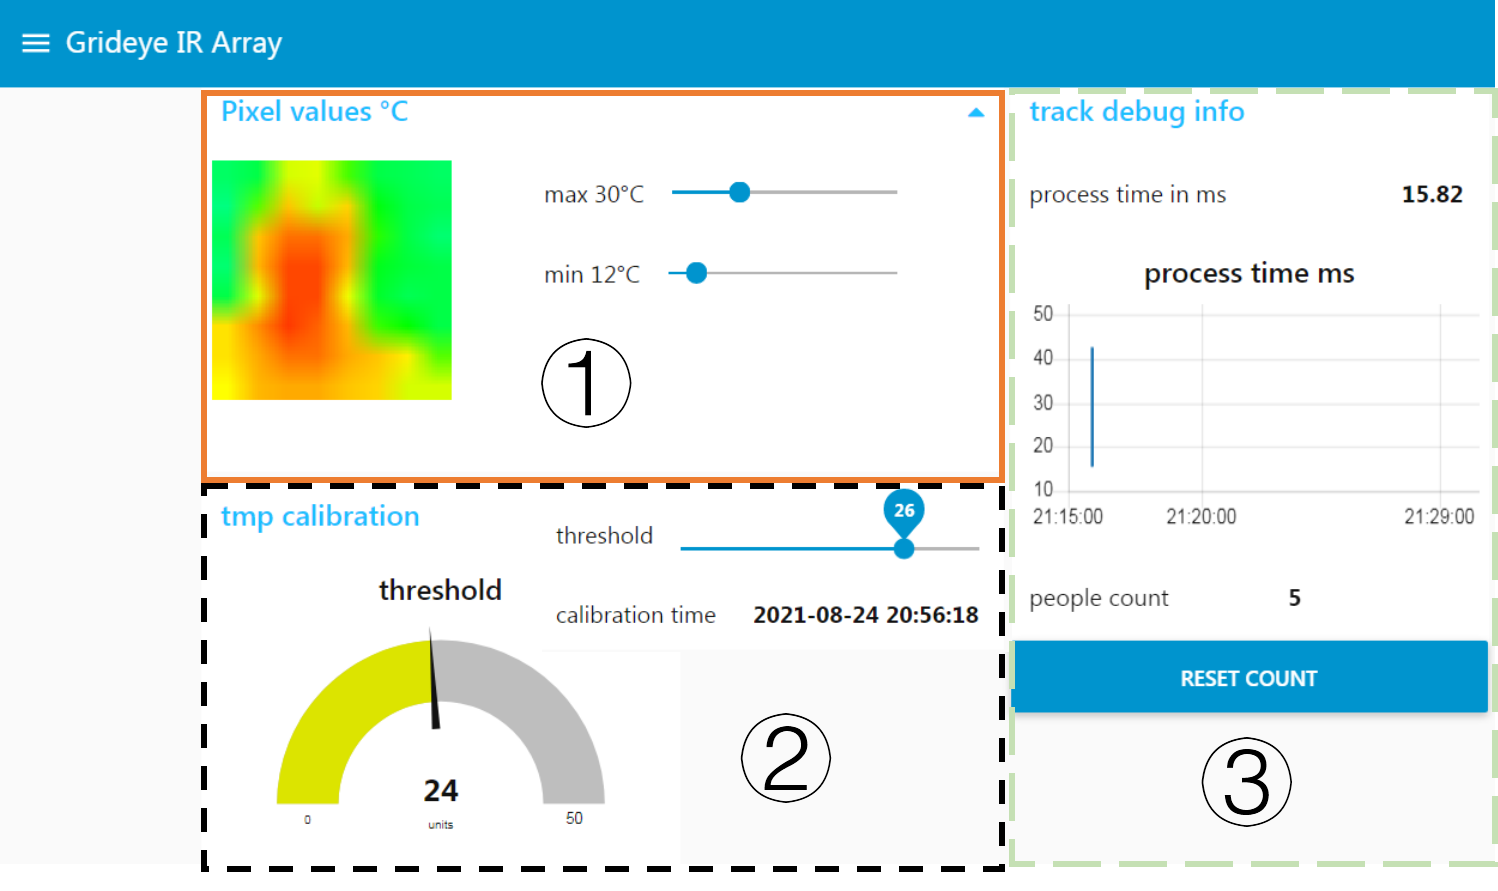
\includegraphics[width=0.8\textwidth]{figures/noderedui.png}
  \caption{Our NodeRed visualization panel is divided into three sections: (1)raw image frame, (2)temperature sensor reading, (3)debug info}\label{fig:noderedui}
\end{figure}

Node-Red has integrated a dashboard which could be used for data visualization. Data in simple format like an integer number or a string, could be visualized with offered presets with no effort. Complicated data like images could be visualized with custom javascript scripts and Angular framework. \autoref{fig:noderedui} shows the dashboard used in our project. The dashboard contains three subsections: region 1 on top-left shows the actual camera view, grayscale pixel values of the IR camera are converted to a heat map, where a redder pixels represents a hotter temperature; region 2 shows the last updated room temperature given by the temperature sensor, which is used for camera calibration, and this value could also be manually assigned; region 3 shows the process time of a single frame and the actual count number, the former is crucial to check whether our algorithm could meet the frame rate constraint, the latter is useful to get an immediate feedback whether the algorithm works properly when we witness an traverse event in region 1.

Besides, Node-Red has a ``file'' node which terminates the flow and stores messages on local storage. We store image files by this way to bypass the MQTT's buffering issue. We don't store images in a data bank because the generated image file size is relative large, about 70Mb every day.
%todo: overview of network dataflow
%
\section{ElasticSearch and Kibana}
To evaluate whether our algorithm outputs the expected relative count, a long-term storage of the count value is needed. For this purpose a data bank based on ElasticSearch and Kibana is used. In ElasticSearch, an individual message is called a ``document'', and a series documents that are similar or generated by a same source are gathered in a group called ``index''. Kibana is a visualization tool combined with ElasticSeearch that can visualize data by indexes. Developed by TUM researchers, the data bank we used has an MQTT interface which receives time-series data, and the accepted message format is one float number and a timestamp. 

In our use case, whenever an entering/ exiting event is detected, a pair of messages, the actual timestamp and the count value at that time will be published and recorded in the data bank. \autoref{fig:ESKibana} shows the recorded data in one afternoon, where the green line is the output of the counting algorithm and the red dots are the ground truth, annotated manually by watching the stored image sequence. Details about ground truth annotation and the evaluation result will be elaborated in \autoref{ch:evaluation}.
\begin{figure}
  \centering
  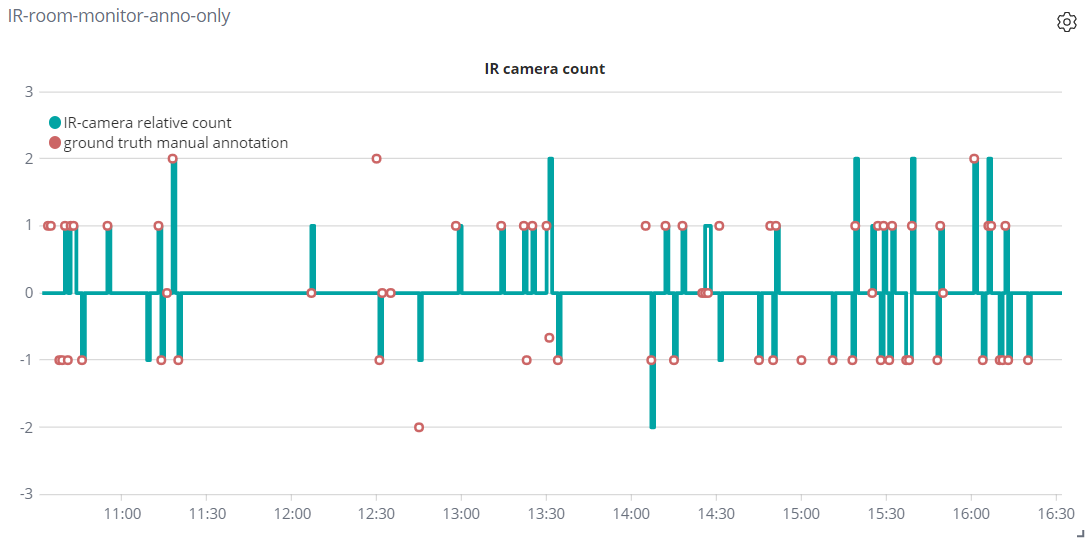
\includegraphics[width=0.8\textwidth]{figures/ESKibana_overview.PNG}
  \caption{A fraction of the recorded data. Green line shows the output of the algorithm and red dots are the ground truth}\label{fig:ESKibana}
\end{figure}


  